%%%%%%%%%%%%%%%%%%%%%%%%%%%%%%%%%%%%%%%%%
% Beamer Presentation
% LaTeX Template
% Version 1.0 (10/11/12)
%
% This template has been downloaded from:
% http://www.LaTeXTemplates.com
%
% License:
% CC BY-NC-SA 3.0 (http://creativecommons.org/licenses/by-nc-sa/3.0/)
%
%%%%%%%%%%%%%%%%%%%%%%%%%%%%%%%%%%%%%%%%%

%----------------------------------------------------------------------------------------
%	PACKAGES AND THEMES
%----------------------------------------------------------------------------------------

\documentclass{beamer}

\mode<presentation> {

% The Beamer class comes with a number of default slide themes
% which change the colors and layouts of slides. Below this is a list
% of all the themes, uncomment each in turn to see what they look like.

%\usetheme{default}
%\usetheme{AnnArbor}
%\usetheme{Antibes}
%\usetheme{Bergen}
%\usetheme{Berkeley}
%\usetheme{Berlin}
%\usetheme{Boadilla}
%\usetheme{CambridgeUS}
\usetheme{Copenhagen}
%\usetheme{Darmstadt}
%\usetheme{Dresden}
%\usetheme{Frankfurt}
%\usetheme{Goettingen}
%\usetheme{Hannover}
%\usetheme{Ilmenau}
%\usetheme{JuanLesPins}
%\usetheme{Luebeck}
%\usetheme{Madrid}
%\usetheme{Malmoe}
%\usetheme{Marburg}
%\usetheme{Montpellier}
%\usetheme{PaloAlto}
%\usetheme{Pittsburgh}
%\usetheme{Rochester}
%\usetheme{Singapore}
%\usetheme{Szeged}
%\usetheme{Warsaw}

% As well as themes, the Beamer class has a number of color themes
% for any slide theme. Uncomment each of these in turn to see how it
% changes the colors of your current slide theme.

%\usecolortheme{albatross}
%\usecolortheme{beaver}
%\usecolortheme{beetle}
%\usecolortheme{crane}
%\usecolortheme{dolphin}
%\usecolortheme{dove}
%\usecolortheme{fly}
%\usecolortheme{lily}
%\usecolortheme{orchid}
%\usecolortheme{rose}
%\usecolortheme{seagull}
%\usecolortheme{seahorse}
%\usecolortheme{whale}
%\usecolortheme{wolverine}

%\setbeamertemplate{footline} % To remove the footer line in all slides uncomment this line
\setbeamertemplate{footline}[page number] % To replace the footer line in all slides with a simple slide count uncomment this line

\setbeamertemplate{navigation symbols}{} % To remove the navigation symbols from the bottom of all slides uncomment this line
}

\usepackage{graphicx} % Allows including images
\usepackage{booktabs} % Allows the use of \toprule, \midrule and \bottomrule in tables

\usepackage{algorithm,algpseudocode}


%----------------------------------------------------------------------------------------
%	TITLE PAGE
%----------------------------------------------------------------------------------------

\title{Amostragem e medidas de qualidade de shapelets} % The short title appears at the bottom of every slide, the full title is only on the title page

\author{Lucas S. Cavalcante} % Your name
\institute[ICMC-USP] % Your institution as it will appear on the bottom of every slide, may be shorthand to save space
{
Instituto de Ci{\^e}ncias Matem{\'a}ticas e de Computa{\c c}{\~a}o, Universidade de S{\~a}o Paulo \\ % Your institution for the title page
\medskip
\textit{Orientador: Gustavo E. A. P. A. Batista} % Your email address
}
\date{\today} % Date, can be changed to a custom date

\begin{document}

\begin{frame}
\titlepage % Print the title page as the first slide
\end{frame}

\begin{frame}
\frametitle{Estrutura}
\tableofcontents
\end{frame}

%--------------------------------------------------------------------------------
%	PRESENTATION SLIDES
%--------------------------------------------------------------------------------

%------------------------------------------------
\section{Defini{\c c}{\~o}es \& Nota{\c c}{\~o}es}
%------------------------------------------------

\begin{frame}
\frametitle{Defini{\c c}{\~o}es \& Nota{\c c}{\~o}es}
\begin{itemize}
\item Uma s{\'e}rie temporal {\'e} uma sequ{\^e}ncia ordenada de valores reais de amostras obtidas em um intervalo fixo. Uma s{\'e}rie de $m$ amostras {\'e} denotada por $T = \{t_{1}, t_{2}, \dots, t_{m} \}$, $t_{i} \in \mathbb{R}$.

\item A partir de uma s{\'e}rie temporal {\'e} possível extrair uma subsequ{\^e}ncia, que {\'e} uma sequ{\^e}ncia continua de amostras de uma s{\'e}rie. Por exemplo, uma subsequ{\^e}ncia de 4 amostras com in{\'i}cio na 5ª amostra de $T$ {\'e} denotada por $S = \{t_{5}, t_{6}, t_{7}, t_{8} \}$. Apesar disso, uma subsequ{\^e}ncia tamb{\'e}m {\'e} uma série temporal.
\end{itemize}
\end{frame}

%------------------------------------------------

\begin{frame}
\frametitle{Defini{\c c}{\~o}es \& Nota{\c c}{\~o}es}
Este trabalho est{\'a} centrado na classifica{\c c}{\~a}o supervisionada de s{\'e}ries temporais:
\begin{itemize}
\item Cada s{\'e}rie temporal $T$ possui um r{\'o}tulo de classifica{\c c}{\~a}o $c$, formando assim uma tupla $\langle T, c \rangle$.
\item Por simplicidade este r{\'o}tulo de classifica{\c c}{\~a}o {\'e} denotado por um inteiro $1 \leq c \leq C$.
\end{itemize}

Um conjunto de $n$ tuplas define um conjunto de dados $CD =\{ \langle T_{1}, c_{1} \rangle, \langle T_{2}, c_{2} \rangle, \dots, \langle T_{n}, c_{n} \rangle \}$.
\end{frame}

%------------------------------------------------

\begin{frame}
\frametitle{Defini{\c c}{\~o}es \& Nota{\c c}{\~o}es}
Neste trabalho s{\~a}o feitas in{\'u}meras compara{\c c}{\~o}es entre duas s{\'e}ries temporais, $S$ e $T$, por meio de uma medida de dissimilaridade denotada por $dist(S, T)$.
\begin{itemize}
\item O conjunto de dist{\^a}ncias de uma s{\'e}rie temporal $S$ {\`a} todas as s{\'e}ries de um $CD$ {\'e} denotado por $D_{S} = \{d_{S,1}, d_{S,2}, \dots, d_{S,n}\}$.
\item Como $d_{S,i} \in \mathbb{R}$ {\'e} poss{\'i}vel denotar $\bar{D_{S}}$ como a m{\'e}dia dessas medidas.
\end{itemize}
Por fim, denotaremos por $CD_{|c_{i}}$ e $D_{S|c_{i}}$ as parti{\c c}{\~o}es desses conjuntos por uma classe $c_{i}$ qualquer, e as suas cardinalidades por $|CD_{|c_{i}}|$ e $|D_{S|c_{i}}|$.
\end{frame}

%------------------------------------------------
\section{Introdu{\c c}{\~a}o}
%------------------------------------------------

\subsection{Motiva{\c c}\~ao}

\begin{frame}
\frametitle{Aplica{\c c}{\~a}o e Classifica{\c c}{\~a}o}
O uso de t{\'e}cnicas de classifica{\c c}{\~a}o de s{\'e}ries temporais tem sido aplicado em diversas {\'a}reas, por exemplo, em bot{\^a}nica foi aplicado {\`a} classifica{\c c}{\~a}o de esp{\'e}cies \cite{Ye:2009do}, enquanto que na industria de manufatura foi aplicado para averiguar a qualidade de produ{\c c}{\~a}o \cite{Patri:2014cd}; al{\'e}m de aplica{\c c}{\~o}es nas {\'a}reas de finan{\c c}as, medicina e entretenimento \cite{xi:2006}.
\end{frame}

%------------------------------------------------

%------------------------------------------------
\subsection{T{\'e}cnicas de Classifica{\c c}{\~a}o}
%------------------------------------------------

\begin{frame}
\frametitle{Classifica{\c c}{\~a}o por kNN}

Apesar da pluralidade de {\'a}reas de aplica{\c c}{\~a}o, a evid{\^e}ncia emp{\'i}rica sugere que o simples classificador de vizinhos mais pr{\'o}ximos (kNN) em conjunto com a medida de dissimilaridade \textit{Dynamic Time Warping} (DTW) tem uma acur{\'a}cia que {\'e} dif{\'i}cil de ser superada \cite{Batista:2013by}. No entanto, esta abordagem tem pontos negativos \cite{Ye:2009do}:

\begin{itemize}
\item Classificador de dif{\'i}cil compreens{\~a}o;
\item Custo elevado para classificar uma nova inst{\^a}ncia.
\end{itemize}
\end{frame}

%------------------------------------------------

\begin{frame}
\frametitle{Shapelets}

Shapelet {\'e} uma primitiva de s{\'e}ries temporais introduzida em 2009 que trata das limita{\c c}{\~o}es mencionadas. Esta primitiva {\'e} uma subsequ{\^e}ncia que de certa forma {\'e} representativa de sua classe \cite{Ye:2009do}.

\begin{figure}
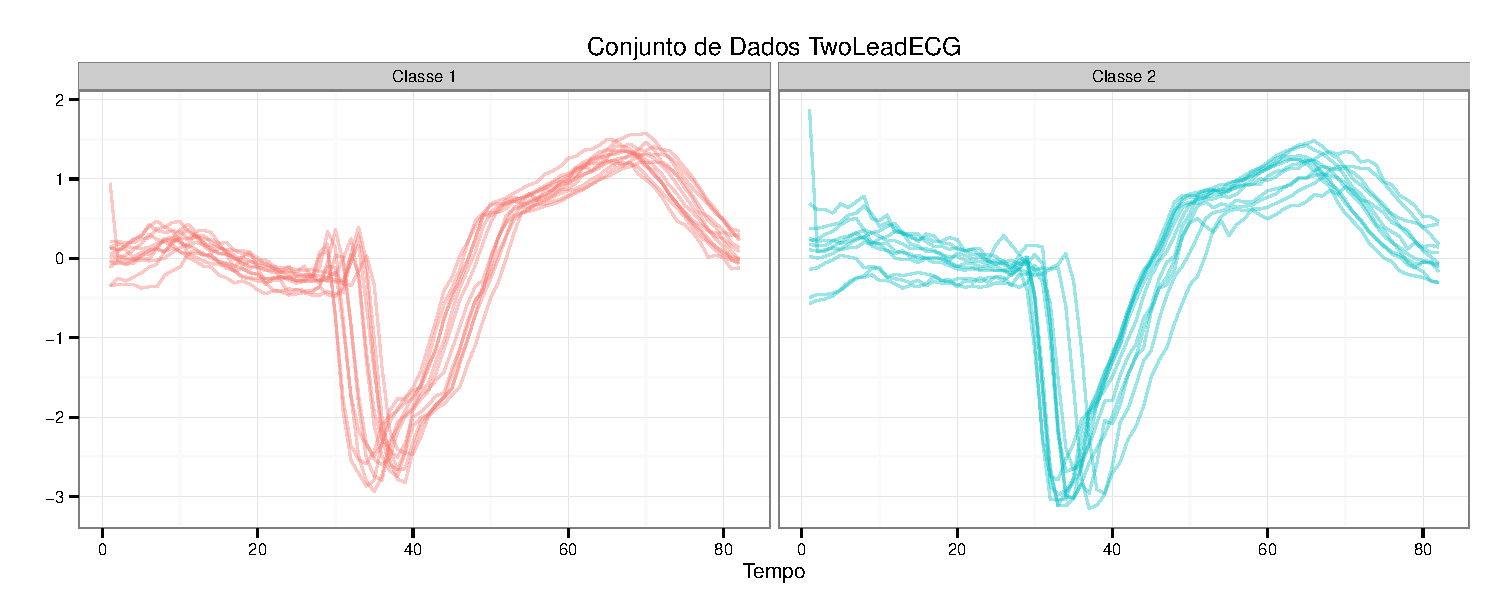
\includegraphics[width=1.0\linewidth]{images/shapelet-exemplo.pdf}
\end{figure}
\end{frame}

%------------------------------------------------

\begin{frame}
\frametitle{{\'A}rvore de Decis{\~a}o Shapelet}

Esta capacidade do shapelet de representar uma classe adv{\'e}m do seu processo de extra{\c c}{\~a}o e avalia{\c c}{\~a}o:

\begin{itemize}
\item Em um conjunto de $n$ s{\'e}ries temporais, cada qual de tamanho $m$, existem $O(nm^{2})$ subsequ{\^e}ncias. Cada uma delas {\'e} um candidato a bom shapelet.

\item A avalia{\c c}{\~a}o dos shapelets se d{\'a} pelo seu ganho de informa{\c c}{\~a}o, que exige a defini{\c c}{\~a}o de uma medida de dissimilaridade entre uma subsequ{\^e}ncia e uma s{\'e}rie temporal.
\end{itemize}

Originalmente esta primitiva foi embutida no classificador de {\'a}rvore de decis{\~a}o, no qual obteve alta acur{\'a}cia, em especial em conjuntos de dados no qual a diferen{\c c}a entre as classes se d{\'a} por padr{\~o}es locais \cite{Ye:2009do}.
\end{frame}

%------------------------------------------------

\begin{frame}
\frametitle{Avalia{\c c}{\~a}o do Shapelet por Medidas de Qualidade}

Intuitivamente, {\'e} question{\'a}vel o uso do ganho de informa{\c c}{\~a}o para avaliar um shapelet em um problema de m{\'u}ltiplas classes, dado que ele prop{\~o}e uma parti{\c c}{\~a}o bin{\'a}ria do conjunto de dados. Por isso, se testou substituir o ganho de informa{\c c}{\~a}o \cite{Lines:2012bv}:

\begin{itemize}
\item Ao se trocar o ganho de informa{\c c}{\~a}o pelas medidas da Mediana de Mood e pelo teste n{\~a}o-param{\'e}trico de Kruskal-Willis, n{\~a}o notou-se nenhuma diferen{\c c}a estatisticamente significativa entre as {\'a}rvores de decis{\~a}o em termos de acur{\'a}cia, por{\'e}m, ao se usar essas outras medidas foi poss{\'i}vel reduzir o tempo de execu{\c c}{\~a}o em at{\'e} quase 20\%.
\end{itemize}
\end{frame}

%------------------------------------------------

\begin{frame}
\frametitle{Transformada Shapelet}

Apesar da boa performance da {\'a}rvore de decis{\~a}o shapelet, um estudo recente mostrou que dissociar o processo de classifica{\c c}{\~a}o do de extra{\c c}{\~a}o de shapelets pode aumentar a acur{\'a}cia \cite{Hills:2013dk}.

\begin{itemize}
\item A dissocia{\c c}{\~a}o {\'e} obtida por construir uma representa{\c c}{\~a}o do conjunto de dados no qual shapelets se tornam atributos que quantificam numericamente uma s{\'e}rie temporal. Esta {\'e} a transformada shapelet.

\item Parte do aumento da acur{\'a}cia adv{\'e}m da possibilidade de usar classificadores mais complexos do que uma {\'a}rvore de decis{\~a}o.
\end{itemize}
\end{frame}

%------------------------------------------------

\begin{frame}
\frametitle{Transformada Shapelet}

Ao se utilizar os classificadores simples de kNN, {\'A}rvore de decis{\~a}o e Naive Bayes e os complexos SVM, Random Forest, Rotation Forest e Bayesian Networks sob a transformada notou-se que \cite{Hills:2013dk}:

\begin{itemize}
\item Em geral, classificadores simples tem uma acur{\'a}cia pior do que os complexos, sendo que o SVM obteve a melhor acur{\'a}cia geral.
\item A conclus{\~a}o {\'e} de que {\'e} prefer{\'i}vel obter a transformada e empregar classificadores complexos, pois se obt{\'e}m uma acur{\'a}cia melhor e a interpretabildiade n{\~a}o {\'e} afetada (os atributos que s{\~a}o os shapelets continuam a serem interpret{\'a}veis).
\end{itemize}

Por{\'e}m, notamos que esses experimentos foram realizados sob um espa{\c c}o reduzido dos shapelets.
\end{frame}

%------------------------------------------------

\begin{frame}
\frametitle{Re-Avalia{\c c}{\~a}o das Medidas de Qualidade}

O trabalho que introduziu a transformada shapelet tamb{\'e}m fez uma re-avalia{\c c}{\~a}o das medidas de qualidade \cite{Hills:2013dk}:

\begin{itemize}
\item Al{\'e}m das medidas alternativas da Mediana de Mood e do teste n{\~a}o-param{\'e}trico de Kruskal-Willis foi adicionada a \textit{f-statistic} utilizada no teste ANOVA.
\item Os experimentos mostraram que a {\'a}rvore de decis{\~a}o com a \textit{f-statistic} possui a maior acur{\'a}cia (sem signific{\^a}ncia estat{\'i}stica) e na m{\'e}dia o menor tempo de execu{\c c}{\~a}o. Com base nesses resultados os autores afirmaram: ``\textit{we argue that the f-statistic should be the default choice for shapelet quality}.''
\end{itemize}

N{\'o}s notamos que os resultados deles vieram de experimentos sob a {\'a}rvore de decis{\~a}o shapelet, mas os autores fizeram tal afirma{\c c}{\~a}o para o caso da transformada shapelet tamb{\'e}m.
\end{frame}

%------------------------------------------------

\begin{frame}
\subsection{Objetivos do Trabalho}
\frametitle{Lacunas \& Objetivos}

\begin{block}{Utilizar todos os shapelets}
Concordamos com a necessidade de se reduzir o espa{\c c}o de busca por bons shapelets por quest{\~o}es de aplica{\c c}{\~o}es pr{\'a}ticas. No entanto, {\'e} necess{\'a}rio ter experimentos que utilizam todos os shapelets para servir como \textit{ground-truth}.
\end{block}

\begin{block}{Utiliza{\c c}{\~a}o de Amostragem Aleat{\'o}ria}
Propor o uso da amostragem aleat{\'o}ria para reduzir o espa{\c c}o de busca por bons shapelets, ao inv{\'e}s de utilizar o algoritmo que restringe a busca por bons shapelets {\`a}queles que tenham um determinado tamanho. Al{\'e}m disso, avaliar como essa redu{\c c}{\~a}o afeta a acur{\'a}cia.
\end{block}
\end{frame}

%------------------------------------------------

\begin{frame}
\frametitle{Lacunas \& Objetivos}
\begin{block}{Avalia{\c c}{\~a}o das Medidas de Qualidade}
Fazer uma extensiva avalia{\c c}{\~a}o das medidas de qualidade sob o dom{\'i}nio da transformada shapelet. Al{\'e}m disso, introduzir uma nova medida de qualidade denominada \textit{in-class transitions} e compar{\'a}-la com as outras duas medidas abordadas neste trabalho: ganho de informa{\c c}{\~a}o e \textit{f-statistic}. A compara{\c c}{\~a}o ser{\'a} em rela{\c c}{\~a}o a acur{\'a}cia.
\end{block}
\end{frame}

%------------------------------------------------
\section{Metodologia}
%------------------------------------------------

%------------------------------------------------

\begin{frame}
\frametitle{Medida de Dissimilaridade}

A medida de Dissimilaridade adotada neste trabalho {\'e} a adapta{\c c}{\~a}o da Dist{\^a}ncia Euclidiana para o caso em que as s{\'e}ries temporais possuem diferentes quantidades de amostras \cite{Ye:2009do}:

\begin{block}{Dist{\^a}ncia Euclidiana entre duas S{\'e}ries Temporais (S, T)}
$dist(S, T) = \underset{\mathrm{0 \leq j < m - m'}}{min} \Bigg\{ \sqrt{\frac{1}{m'}\sum_{i = 1}^{m'}(s_{i} - t_{i + j})^{2}} \Bigg\}$
\end{block}

Com a observa{\c c}{\~a}o de que sempre {\'e} realizada a z-normaliza{\c c}{\~a}o.
\end{frame}

%------------------------------------------------

\begin{frame}
\frametitle{Shapelet}

\begin{itemize}
\item Shapelet {\'e} uma subsequ{\^e}ncia que {\'e} representativa de uma classe.
\item Inicialmente o shapelet era a subsequ{\^e}ncia de maior ganho de informa{\c c}{\~a}o \cite{Ye:2009do}, mas com a transformada shapelet esta defini{\c c}{\~a}o {\'e} relaxada para qualquer subsequ{\^e}ncia que tenha uma medida de qualidade associada a ela.
\item Em um conjunto de dados existem $O(nm^{2})$ shapelets.
\end{itemize}
\end{frame}

%------------------------------------------------

\begin{frame}
\frametitle{Shapelet: Medida de Qualidade}

Seja um shapelet $Sh$ do qual se obteve $D_{Sh}$, ent{\~a}o:

\begin{itemize}
\item \textbf{Ganho de Informa{\c c}{\~a}o:} inicialmente se computa a entropia do conjunto de dados corrente, ent{\~a}o por um corte bin{\'a}rio se particiona este conjunto dois. O ganho de informa{\c c}{\~a}o {\'e} a diferen{\c c}a entre a entropia inicial e a entropia m{\'e}dia das parti{\c c}{\~o}es resultantes \cite{quinlan1992c4}.
\item \textbf{F-Statistic:} {\'e} a mesma m{\'e}trica utilizada no teste da ANOVA (\textit{Analysis of Variance}) para testar a hip{\'o}tese nula de que as m{\'e}dias de todas as classes s{\~a}o iguais.
\begin{block}{C{\'a}lculo da F-Statistic}
$FStatistic(D_{Sh}) = \frac{\sum_{i = 1}^{C}(\bar{D_{Sh | c_{i}}} - \bar{D_{Sh}})^{2} / (C - 1)}{\sum_{i = 1}^{C} \sum_{d_{j} \in D_{Sh | c_{i}}} (d_{j} - \bar{D_{Sh | c_{i}}})^{2} / (n - C)}$
\end{block}
\end{itemize}
\end{frame}

%------------------------------------------------

\begin{frame}
\frametitle{Shapelet: Medidas de Qualidade}

\begin{itemize}
\item \textbf{In-Class Transitions:} {\'e} a contagem de quantos elementos da mesma classe aparecem na ordena{\c c}{\~a}o de $D_{Sh}$.

\begin{figure}
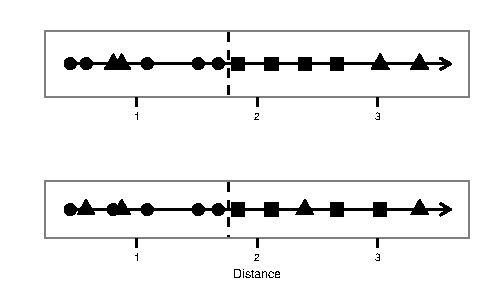
\includegraphics[width=0.7\linewidth]{images/in-class-transitions.pdf}
\end{figure}
\end{itemize}

N{\~a}o importa a medida de qualidade, quanto maior seu valor melhor.
\end{frame}

%------------------------------------------------

\begin{frame}
\frametitle{Shapelets: Sele{\c c}{\~a}o}

Dado um conjunto de shapelets {\'e} preciso selecionar $k$ deles, pois usar todos pode causar overfitting. Um m{\'e}todo naive seria de simplesmente selecionar os $k$ melhores, por{\'e}m, isso pode levar a alta redund{\^a}ncia de atributos.

\begin{figure}
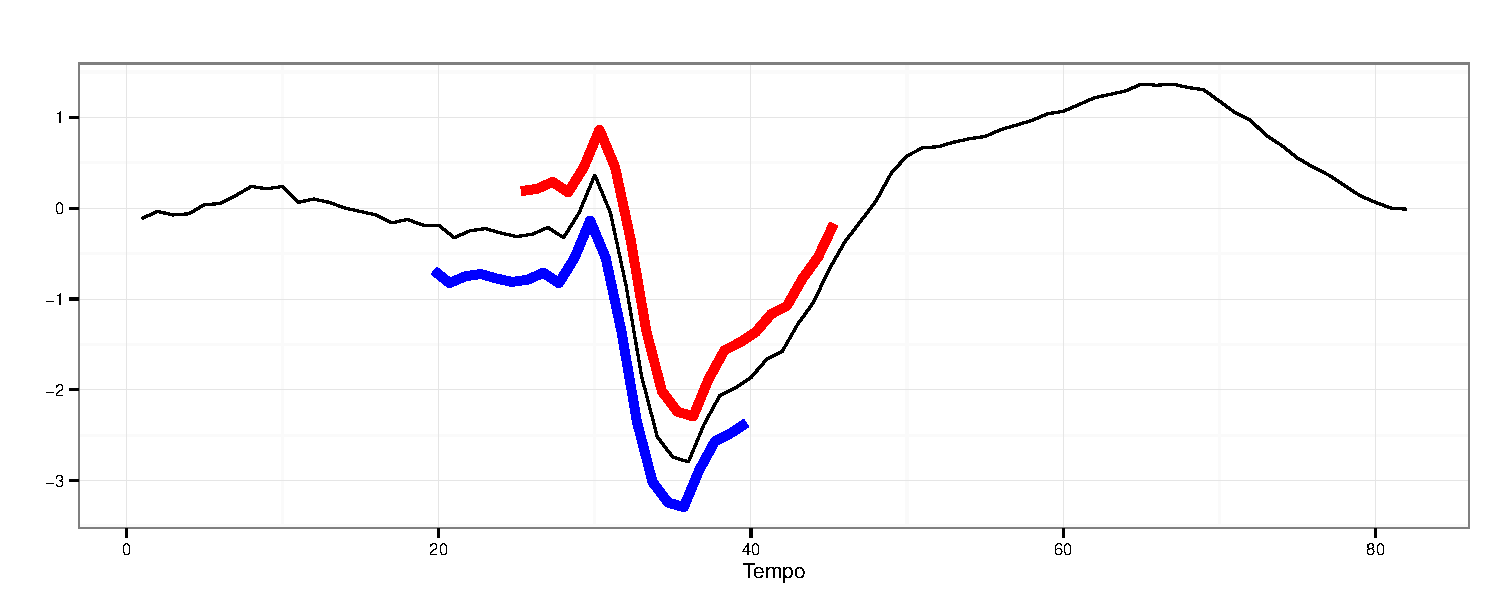
\includegraphics[width=0.7\linewidth]{images/shapelets-similares.pdf}
\end{figure}

Hills et. al \cite{Hills:2013dk} contorna esse problema por definir a auto-similaridade de shapelets.
\end{frame}

%------------------------------------------------

\begin{frame}
\frametitle{Shapelets: Sele{\c c}{\~a}o}
\begin{algorithmic}
\small
\Function{SelecionarKShapelets}{shapelets, k}
	\State selecionados $\leftarrow$ $\emptyset$
    \State Ordenar(shapelets, ``decrescente'', ``medida de qualidade'')
    \For{shapelet $\in$ shapelets}
    	\If{NaoAutoSimilar(shapelet, selecionados)}
        	\State selecionados $\leftarrow$ selecionados $\cup$ shapelet
            \State $k$ $\leftarrow$ $k - 1$
        \EndIf
        
        \If{$k = 0$}
        	\State \Return selecionados
        \EndIf
    \EndFor
    
    \State \Return selecionados
\EndFunction
\end{algorithmic}
\end{frame}

%------------------------------------------------

\begin{frame}
\frametitle{Shapelets: Extra{\c c}{\~a}o}

\begin{itemize}
\item Extra{\c c}{\~a}o de todos os $O(nm^{2})$ shapelets.
\item Extra{\c c}{\~a}o de uma amostragem aleat{\'o}ria dos shapelets.
\item Extra{\c c}{\~a}o de todos os shapelets dentre $min$ e $max$ \cite{Hills:2013dk}:

\begin{algorithmic}
\small
\Function{EstimarMinMax}{$CD$}
	\State shapelets $\leftarrow$ $\emptyset$
    \For{$i\gets 1, 10$}
    	\State subset $\leftarrow$ SelecaoAleatoria($CD$, 10)
    	\State tmp $\leftarrow$ GerarShapelets(subset, 3, $m$)
        \State shapelets $\leftarrow$ shapelets $\cup$ SelecionrKShapelets(tmp, 10)
    \EndFor

    \State Ordenar(shapelets, ``crescente'', ``tamanho'')
    \State min $\leftarrow$ shapelets[25]
    \State max $\leftarrow$ shapelets[75]
    \State \Return min, max
\EndFunction
\end{algorithmic}
\end{itemize}
\end{frame}

%------------------------------------------------

\begin{frame}
\frametitle{Shapelets: Transformada}

Ap{\'o}s a extra{\c c}{\~a}o dos shapelets e a compurta{\c c}{\~a}o de sua qualidade, ent{\~a}o se escolhe $k$ shapelets para compor o grupo de atributos $Sh$. Na transformada shapelet cada s{\'e}rie temporal {\'e} representada pela sua dist{\^a}ncia aos shapelets em $Sh$.

\begin{table}
\centering
\small
\caption{Descri{\c c}{\~a}o da transformada shapelet. Cada linha representa uma s{\'e}rie temporal e cada coluna um shapelet, com uma coluna extra para o r{\'o}tulo de classifica{\c c}{\~a}o. Cada $a_{ij}$ {\'e} a dist{\^a}ncia entre um shapelet {\'e} uma s{\'e}rie temporal.}
\label{tab-shapelet-transform}
\begin{tabular}{c | c c c c c}
Time Series & $Sh_{1}$ & $Sh_{2}$ & $\ldots$ & $Sh_{k}$ & Class. Label \\ \hline
$T_{1}$ & $a_{11}$ & $a_{12}$ & $\ldots$ & $a_{1k}$ & $c_{1}$ \\
$T_{2}$ & $a_{21}$ & $a_{22}$ & $\ldots$ & $a_{2k}$ & $c_{2}$ \\
$\vdots$ & $\vdots$ & $\vdots$ & $\ddots$ & $\vdots$ & $\vdots$ \\
$T_{n}$ & $a_{n1}$ & $a_{n2}$ & $\ldots$ & $a_{nk}$ & $c_{n}$ \\ \hline
\end{tabular}
\end{table}
\end{frame}

%------------------------------------------------

\begin{frame}
\frametitle{Shapelets: Classifica{\c c}{\~a}o}

Uma vez que se saiba obter a transformada shapelet de um $CD$, ent{\~a}o para classificar novas s{\'e}ries temporais a partir de um conjunto de treinamento basta:

\begin{enumerate}
\item Obter a transformada shapelet do conjunto de treinamento.
\item Induzir um modelo de classifica{\c c}{\~a}o sob tal transformada.
\item Obter a transformada shapelet do conjunto de teste.
\item Executar o modelo de classifica{\c c}{\~a}o usando como entrada a transformada do conjunto de teste.
\end{enumerate}

Neste trabalho ser{\~a}o explorados os seguintes classificadores: kNN, Random Forest e Support Vector Machines (SVM).

\end{frame}

%------------------------------------------------
\section{Experimentos \& Resultados}
%------------------------------------------------

%------------------------------------------------
\subsection{Arranjo Experimental}
\begin{frame}
\frametitle{Arranjo Experimental}
\begin{itemize}
\item Os experimentos foram executados em um Intel Core i7 @ 2.3GHz.
\item A linguagem utilizada neste trabalho foi a R. Por{\'e}m, para executar os experimentos em um tempo razo{\'a}vel, foi feita a paraleliza{\c c}{\~a}o e uso da linguagem C++ por meio do pacote RcppParallel.
\item Todos os experimentos foram executados em uma cole{\c c}{\~a}o de 28 conjuntos de dados do reposit{\'o}rio da UCR \cite{UCRArchive}.
\end{itemize}

Com o detalhe de que a quantidade de atributos, em nossos experimentos, {\'e} dependente da quantidade de classes de cada conjunto de dados.
\end{frame}

%------------------------------------------------
\subsection{Experimentos: Medida de Qualidade}
\begin{frame}
\frametitle{Avalia{\c c}{\~a}o de Acur{\'a}cia das Medidas de Qualidade}

\begin{figure}
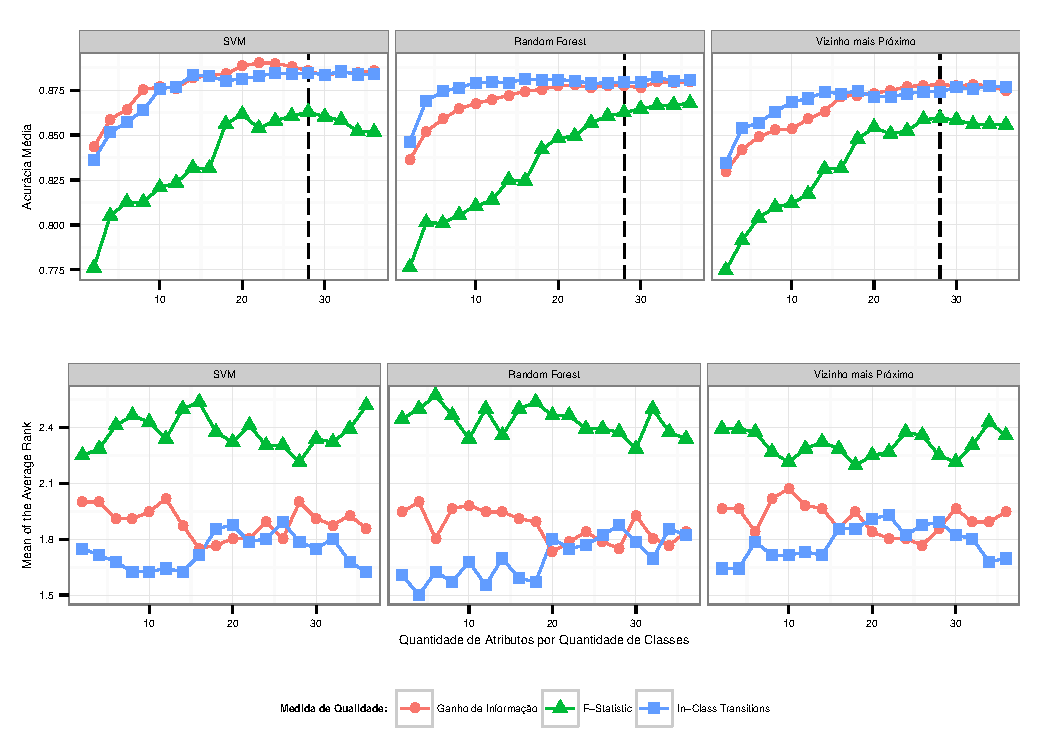
\includegraphics[width=0.85\linewidth]{images/accuracy-quality.pdf}
\end{figure}
\end{frame}

%------------------------------------------------
\subsection{Experimentos: Redu{\c c}{\~a}o do Espa{\c c}o de Busca}
\begin{frame}
\frametitle{Avalia{\c c}{\~a}o da Amostragem Aleat{\'o}ria}

\begin{figure}
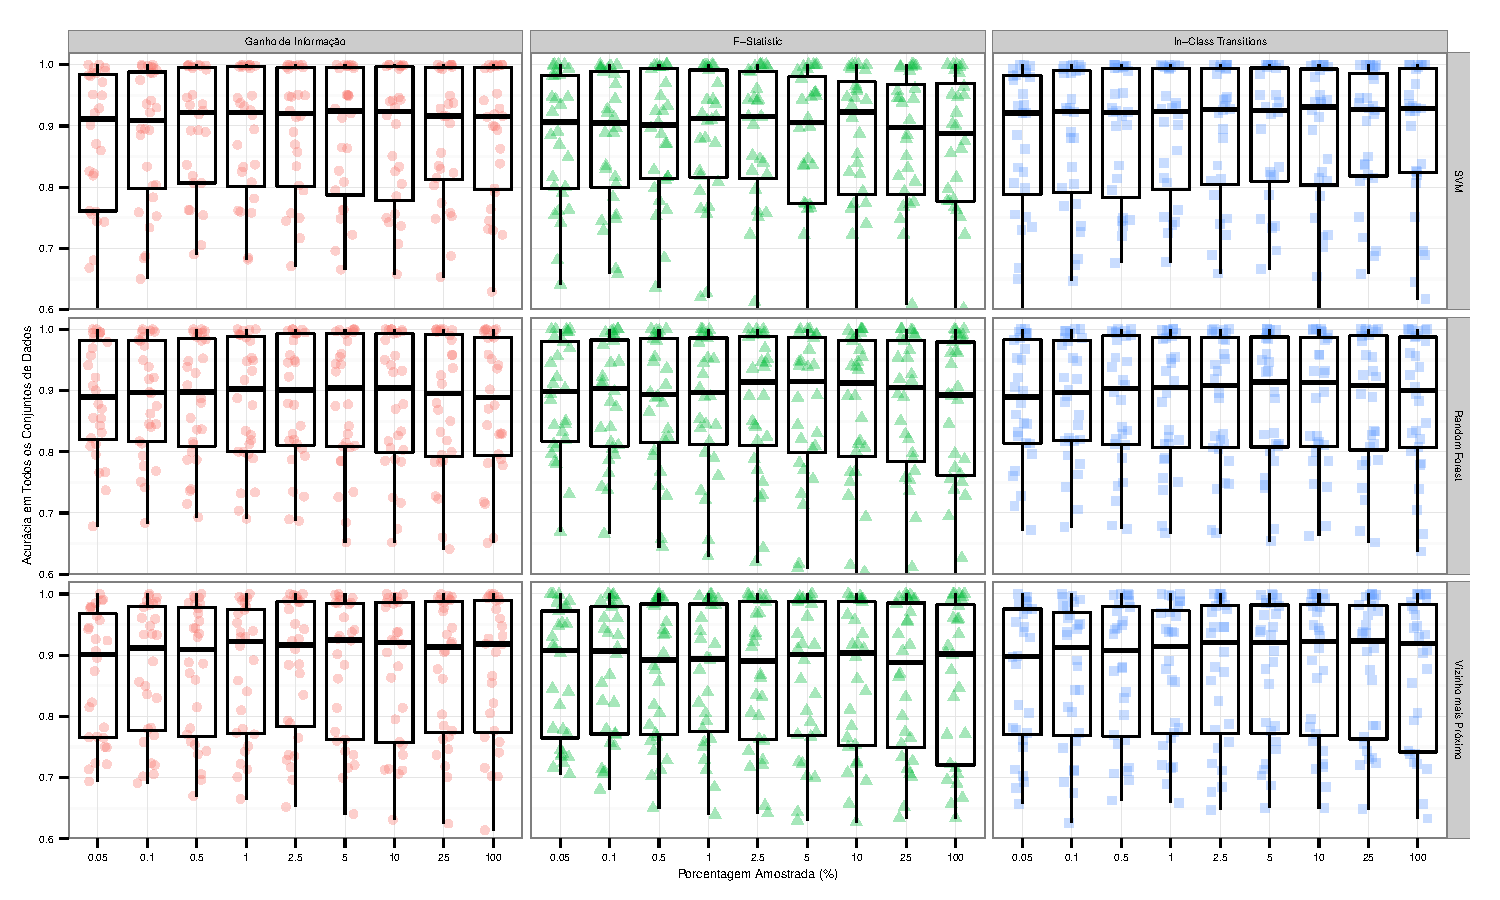
\includegraphics[width=1.0\linewidth]{images/random-sampling.pdf}
\end{figure}
\end{frame}

%------------------------------------------------
\begin{frame}
\frametitle{Comparativo entre as T{\'e}cnicas de Redu{\c c}{\~a}o do Espa{\c c}o}

\begin{figure}
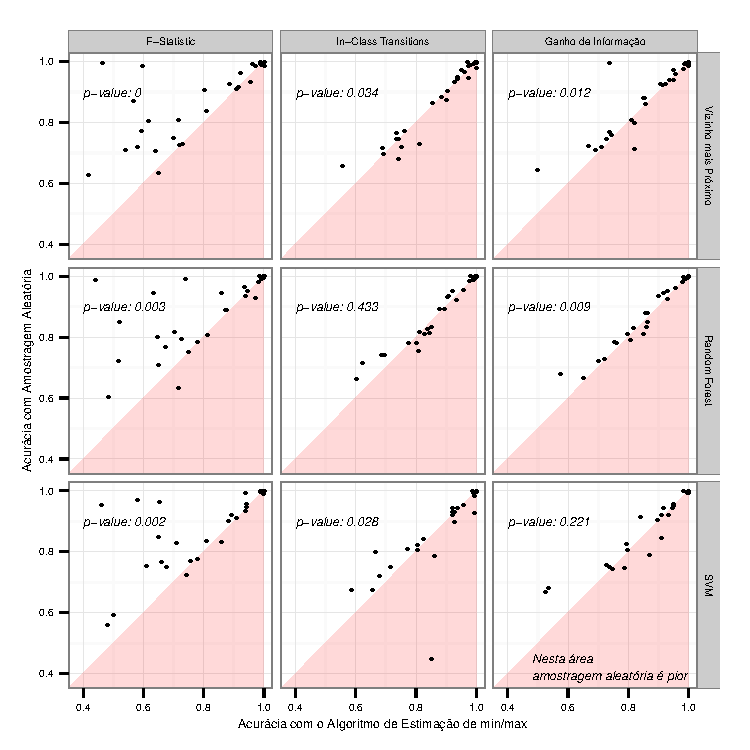
\includegraphics[width=0.6\linewidth]{images/random-sampling-vs.pdf}
\end{figure}
\end{frame}

%------------------------------------------------
\begin{frame}
\frametitle{Comparativo entre as T{\'e}cnicas de Redu{\c c}{\~a}o do Espa{\c c}o}

\begin{table}
\centering
\small
\caption{O algoritmo \texttt{EstimarMinMax()} estima uma faixa de valores de tamanho do qual todos os shapelets s{\~a}o extra{\'i}dos. Dessa estima{\c c}{\~a}o calculamos o percentual que essa faixa representa do todo, ent{\~a}o sumarizamos essa informa{\c c}{\~a}o pelos quantis (5 execu{\c c}{\~o}es para cada conjunto de dados).}
\label{tab-quantiles-algorithm}
\begin{tabular}{r|ccc}
\hline
	& Ganho de Informa{\c c}{\~a}o & F-Stat & In-Class Transitions\\ \hline
M{\'i}nimo (\%) & 25,7 & 1,558 & 20,11 \\
$1^{o}$ Quartil (\%) & 31,51 & 10,56 & 31,3 \\
Mediana (\%) & 35,31 & 16,08 & 36,52 \\
M{\'e}dia (\%) & 37,24 & 18,28 & 36,28 \\
$3^{o}$ Quartil (\%) & 43,94 & 27,81 & 41,76 \\
M{\'a}ximo (\%) & 56,09 & 40,26 & 49,08 \\
\hline
\end{tabular}
\end{table}
\end{frame}

%------------------------------------------------
\subsection{Experimentos: Compara{\c c}{\~a}o com o modelo de Hills et. al}
\begin{frame}
\frametitle{Compara{\c c}{\~a}o com o modelo de Hills et. al \cite{Hills:2013dk}}

\begin{figure}
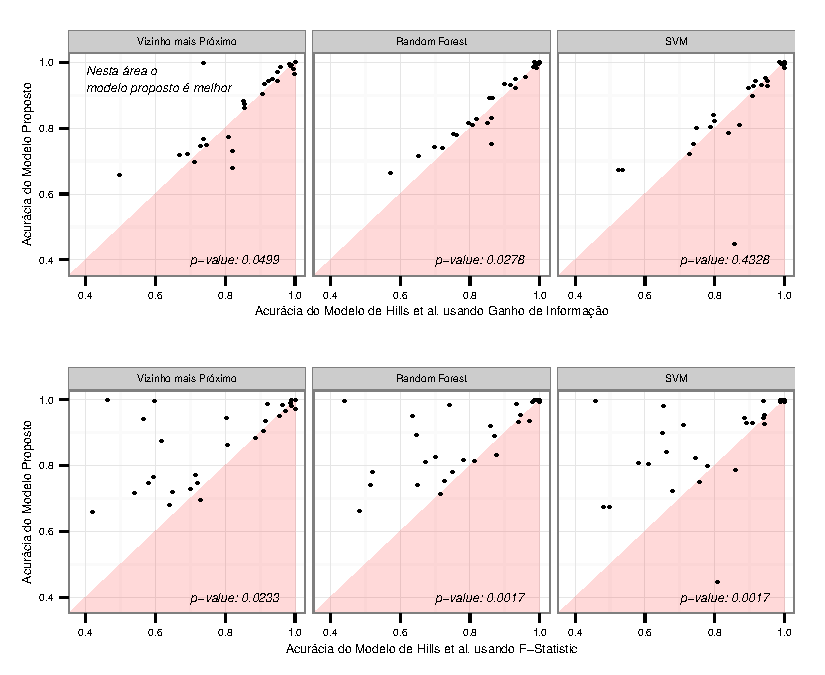
\includegraphics[width=0.75\linewidth]{images/final-comparison.pdf}
\end{figure}
\end{frame}

%------------------------------------------------
\section{Conclus{\~a}o \& Trabalhos Futuros}
%------------------------------------------------

\begin{frame}
\frametitle{Conclus{\~a}o \& Trabalhos Futuros}
\begin{itemize}
\item Em nossa an{\'a}lise sobre as medidas de qualidade os nossos achados contradizem a recomenda{\c c}{\~a}o pr{\'e}via do uso da f-statistic, pois ela obeteve a pior performance. 

\begin{itemize}
\item A nossa medida proposta, denominada in-class transitions, possui a melhor performance, especialmente quando poucos atributos s{\~a}o utilizados. Quando mais atributo s{\~a}o utilizados a sua performance se torna pr{\'o}xima a de ganho de informa{\c c}{\~a}o. 

\item Apesar da in-class transitions ser de f{\'a}cil comprees{\~a}o e de implementa{\c c}{\~a}o ela ainda requer a ordena{\c c}{~a}o dos elementos, logo, dever{\'a} ser mais lenta que a f-statistic, por{\'e}m mais r{\'a}pida do que a de ganho de informa{\c c}{\~a}o.
\end{itemize}
\end{itemize}
\end{frame}

%------------------------------------------------

\begin{frame}
\frametitle{Conclus{\~a}o \& Trabalhos Futuros}
\begin{itemize}
\item Como em um conjunto de dados existem $O(nm^{2})$ shapelets, a computa{\c c}{\~a}o de todos pode ser impratic{\'a}vel, logo m{\'e}todos que reduzam o espa{\c c}o de buscam se tornam uma necessidade.

\begin{itemize}
\item O trabalho de Hills et al \cite{Hills:2013dk} sugere o uso de algoritmo \texttt{EstimarMinMax()} que restringe a busca por bons shapelets {\`a}queles que tenham um determinado tamanho, enquanto que n{\'o}s propusemos o uso de amostragem aleat{\'o}ria.

\item Nossos experimentos mostraram que o uso de \texttt{EstimarMinMax()} introduz um overhead significativo sem no entanto reduzir o espa{\c c}o de busca de forma eficiente.

\item O uso de amostragem aleat{\'o}ria mostrou que pode oferecer um pequeno aumento da acur{\'a}cia e diminui{\c c}{\~a}o de sua variabilidade. Supomos que isso de em raz{\~a}o de uma maior diversidade dos atributos.
\end{itemize}
\end{itemize}
\end{frame}

%------------------------------------------------

\begin{frame}
\frametitle{Conclus{\~a}o \& Trabalhos Futuros}
\begin{itemize}
\item N{\'o}s esperamos que as {\'a}reas de redu{\c c}{\~a}o de espa{\c c}o de busca e de prover maior diversidade nos shapelets recebam maior aten{\c c}{\~a}o no futuro. Por enquanto a nossa contribui{\c c}{~a}o se restringe a recomendar o uso da amostragem aleat{\'o}ria como o baseline para ambas as {\'a}reas.
\end{itemize}
\end{frame}

%------------------------------------------------
\section{Agradecimentos}
%------------------------------------------------

\begin{frame}
\frametitle{Agradecimentos}
Agradecimentos ao Daniel Y. T. Chino por sua sugest{\~a}o de uso de amostragem aleat{\'o}ria para shapelets; e a FAPESP que financiou este trabalho (2013/16164-2)

\begin{figure}

\includegraphics[width=0.7\linewidth]{images/fapesp.png}
\end{figure}
\end{frame}

%------------------------------------------------

\begin{frame}[allowframebreaks] 
\frametitle{Refer{\^e}ncias}
\footnotesize{
\begin{thebibliography}{99}
\bibitem{Ye:2009do}
Lexiang Ye and Eamonn Keogh.
\newblock {Time series shapelets: a new primitive for data mining}.
\newblock In {\em {Proceedings of the 15th ACM SIGKDD international conference
  on Knowledge discovery and data mining}}, pages {947--956}. ACM, 2009.

\bibitem{Patri:2014cd}
Om~P Patri, Abhishek~B Sharma, Haifeng Chen, Guofei Jiang, Anand~V Panangadan,
  and Viktor~K Prasanna.
\newblock {Extracting discriminative shapelets from heterogeneous sensor data}.
\newblock In {\em {Big Data (Big Data), 2014 IEEE International Conference
  on}}, pages 1095--1104. {IEEE}, 2014.
  
\bibitem{xi:2006}
Xiaopeng Xi, Eamonn Keogh, Christian Shelton, Li Wei and Chotirat Ann Ratanamahatana.
\newblock {Fast time series classification using numerosity reduction}.
\newblock In {\em {Proceedings of the 23rd international conference on Machine learning}}, pages {1033--1040}. ACM, 2006.

\bibitem{Batista:2013by}
Gustavo~EAPA Batista, Eamonn~J Keogh, Oben~Moses Tataw, and Vin{\'\i}cius~MA
  de~Souza.
\newblock {CID: an efficient complexity-invariant distance for time series}.
\newblock {\em Data Mining and Knowledge Discovery}, 28(3):{634--669}, 2014.

\bibitem{Lines:2012bv}
Jason Lines and Anthony Bagnall.
\newblock {Alternative quality measures for time series shapelets}.
\newblock In {\em {Intelligent Data Engineering and Automated Learning-IDEAL
  2012}}, pages {475--483}. {Springer}, 2012.

\bibitem{Hills:2013dk}
Jon Hills, Jason Lines, Edgaras Baranauskas, James Mapp, and Anthony Bagnall.
\newblock {Classification of time series by shapelet transformation}.
\newblock {\em Data Mining and Knowledge Discovery}, 28(4):851--881, 2014.

\bibitem{quinlan1992c4}
Ross~J Quinlan.
\newblock C4. 5: Programs for machine learning.
\newblock 1992.

\bibitem{UCRArchive}
Yanping Chen, Eamonn Keogh, Bing Hu, Nurjahan Begum, Anthony Bagnall, Abdullah
  Mueen, and Gustavo Batista.
\newblock The ucr time series classification archive, July 2015.
\newblock \url{www.cs.ucr.edu/~eamonn/time_series_data/}.
\end{thebibliography}
}
\end{frame}

%----------------------------------------------------------------------------------------

\end{document}